\lecture{12}{22 Oct. 13:20}{}
\begin{prev}
    We have learnt that 
    \[
        \left\{ \text{Conjugacy classes of } S_n  \right\} = \left\{ \text{cycle types } (1)^{v_1}(2)^{v_2}\dots \text{ with } 1 \cdot v_1 + 2 \cdot v_2 + \dots = n   \right\}.  
    \]
    Also, we know 
    \[
        \left\vert (1)^{v_1} (2)^{v_2} \dots  \right\vert = \frac{n!}{1^{v_1} v_1 ! 2^{v_2} v_2 ! \dots }. 
    \]
    Besides, we have learnt that 
    \[
        H \triangleleft G \iff H \text{ is a union of conj classes of } G \text{ i.e. } H = \bigcup_{x \in H} C(x).   
    \]
\end{prev}

\begin{figure}[H]
    \centering
    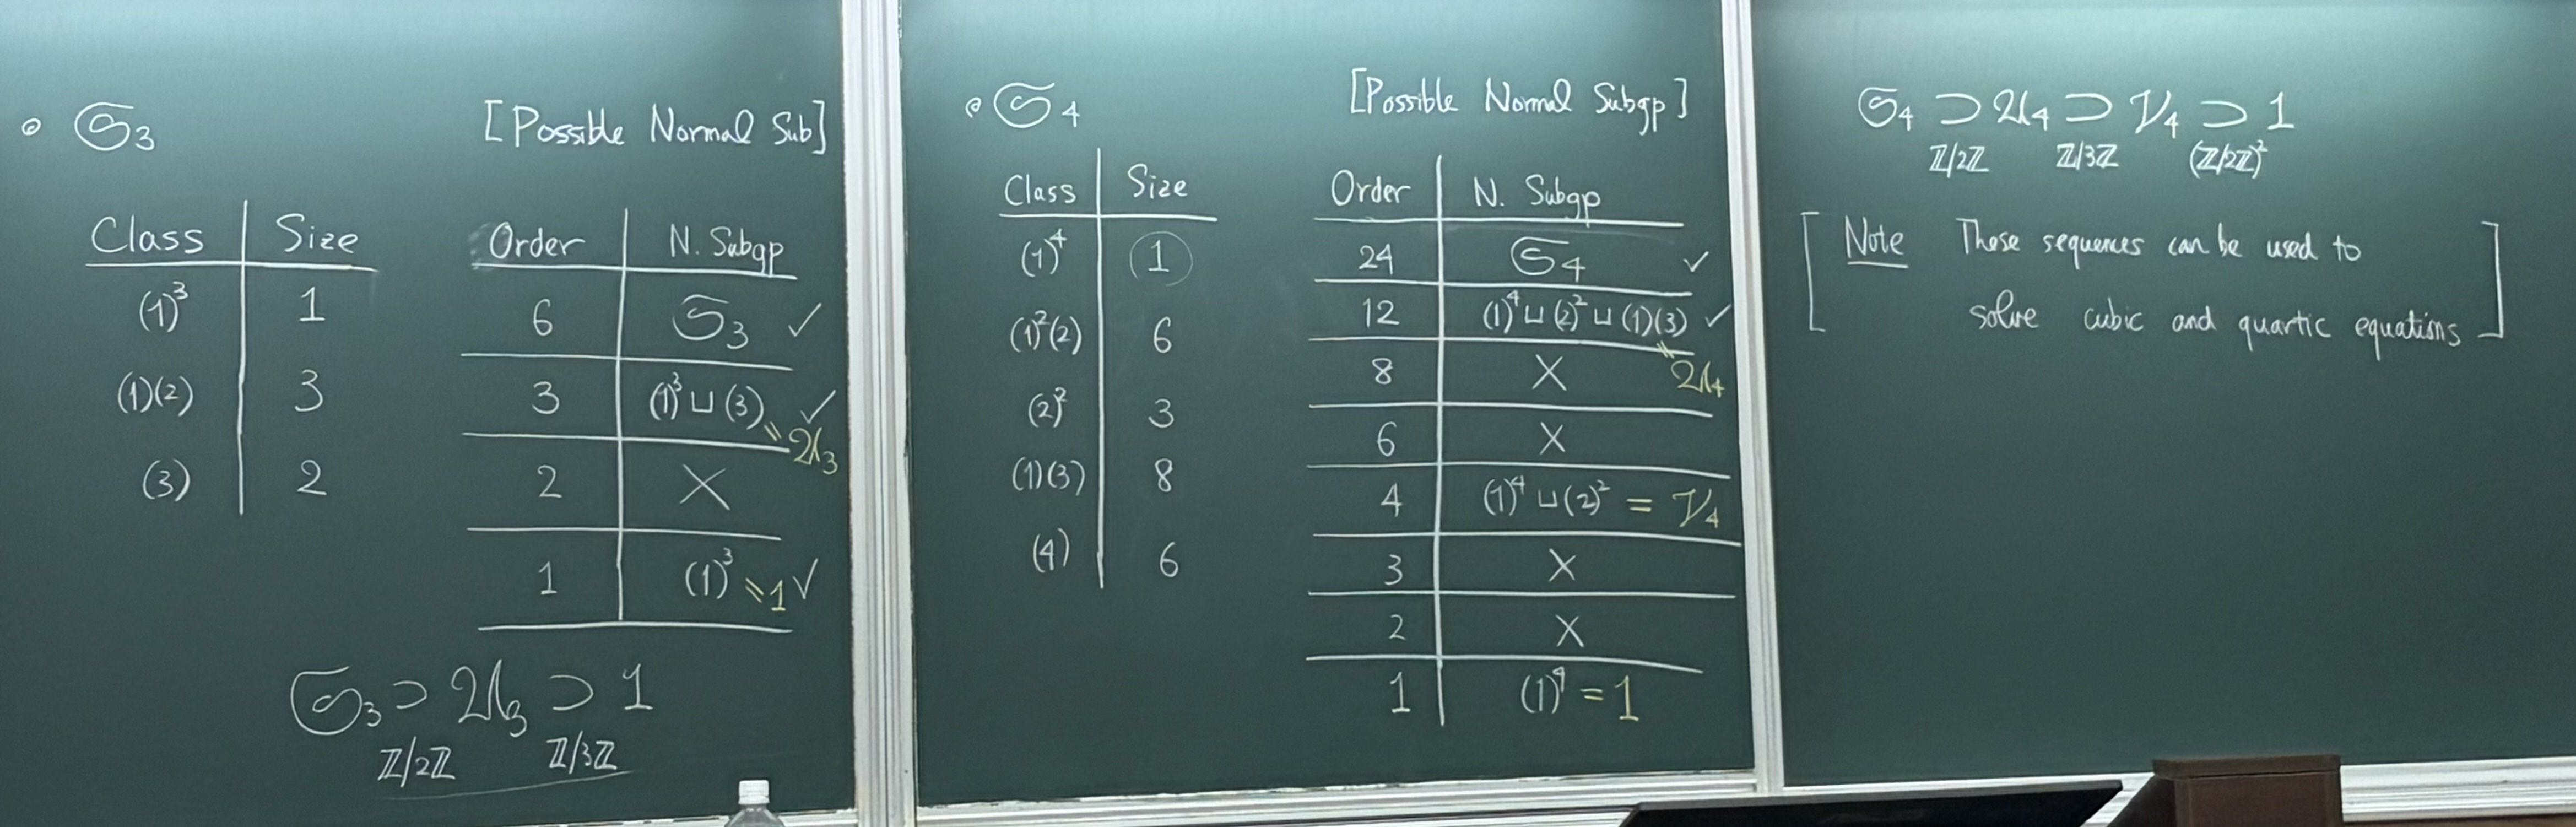
\includegraphics[width=\textwidth]{./Figures/PossibleNormalSubgroup.jpg}
    \caption{Possible normal subgroups of \(S_3\) and \(S_4\)}
    \label{fig:PossibleNormalSubgroup}
\end{figure}

\begin{remark}
    Since we know \(H\) is a normal subgroup of \(S_n\) iff \(H = \bigcup_{x \in H} C(x) \), where \(C(x)\) is the conjugacy class of \(S_n\), and conjugacy classes of symmetric groups are the sets of permutations of same cycle form, and since the size of a subgroup of \(S_n\) must divide \(\vert S_n \vert = n!\), so we can deduce all normal subgroups of \(S_n\).     
\end{remark}

\begin{definition}[Transpositions]
    We say a permutation \(\pi \in S_n \) is a transposition iff \(\pi \in (1)^{n-2}(2)\).  
\end{definition}

\begin{theorem}
    Every \(\sigma \in S_n\) is a product of transpositions. More specifically, this argument holds with adjacent transpositions. 
\end{theorem}

\begin{proof}
    Since \(\sigma \) can be factored into independent cyclic permutations, so we just need to show any cyclic permutation is a product of transpositions. Suppose we have 
    \[
        \tau = \begin{pmatrix}
            a_1 & a_2 & \dots  & a_n  \\
            a_2 & a_3 & \dots  & a_1  \\
        \end{pmatrix},
    \] then we have:
    \[
        (a_1 a_2) (a_2 a_3) \dots (a_{n-1} a_n) I_n = \tau .
    \]
    Note that we first operate \((a_1 a_2)\), then \((a_2 a_3)\), and so on.
    
    Actually, if we do bubble sort on \(\sigma \), then it can becomes \(I_n\), then we can do the inverse operation to make \(I_n\) go back to \(\sigma \), so \(\sigma \) is just the product of adjacent transpositions.     
\end{proof}

%Ladder Lottery
\begin{figure}[H]
    \centering
    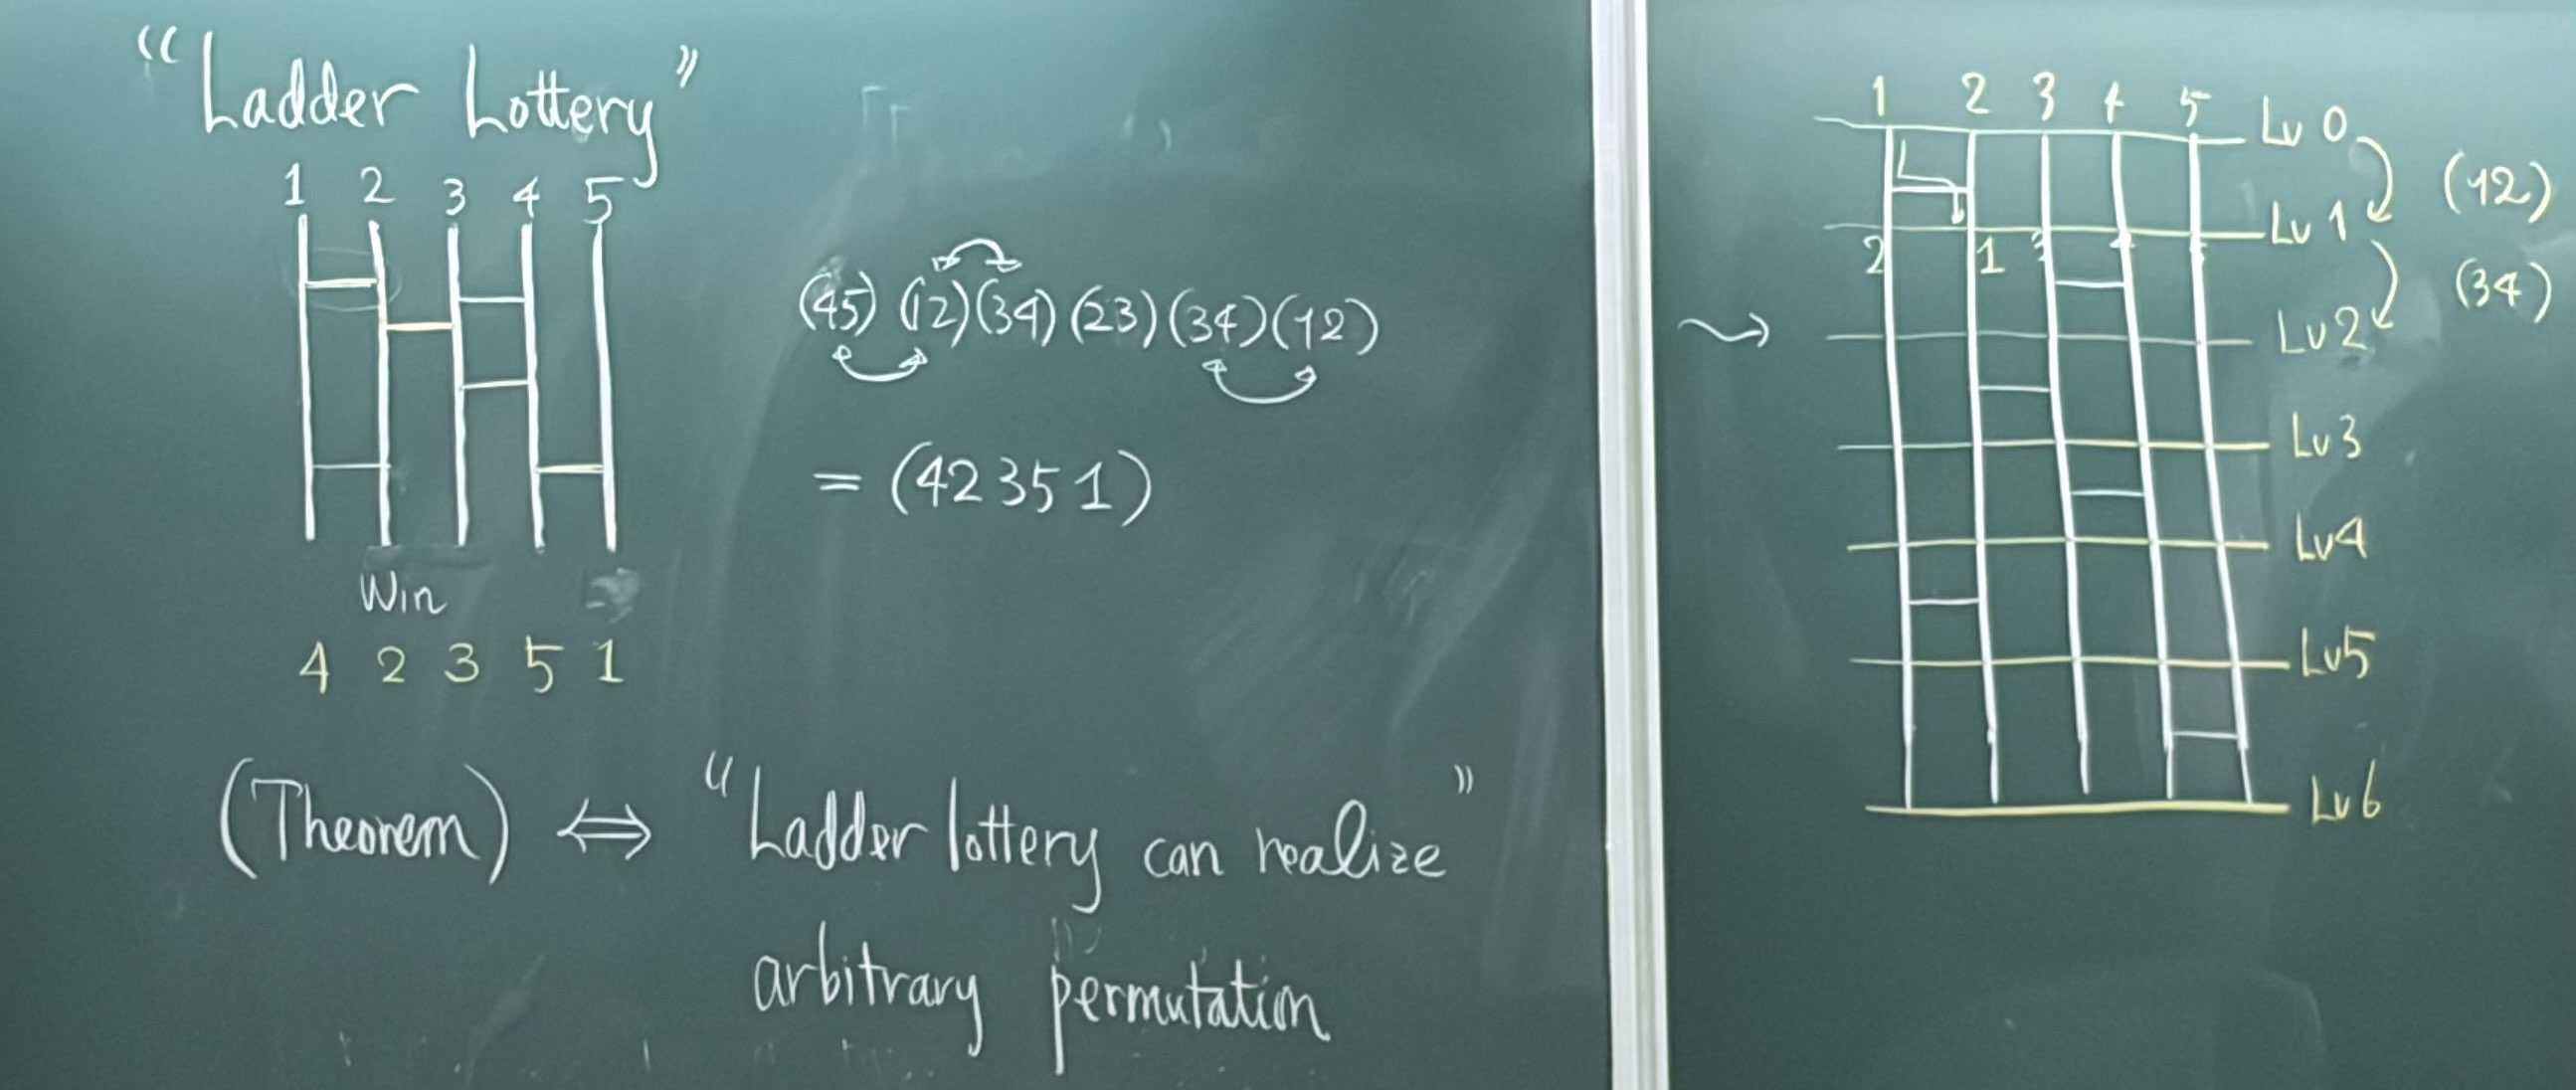
\includegraphics[width=\textwidth]{./Figures/LadderLottery.jpg}
    \caption{Ladder Lottery can realize arbitrary permutations}
    \label{fig:Ladder Lottery}
\end{figure}
\begin{remark}
    In ladder lottery, whenever we meet a bridge, we must go through it no matter we go left or go right, so every bridge is a (adjacent) transposition, and since every permuatation can be decomposed into adjacent transpositions, so ladder lottery can realize all permutations.
\end{remark}
%────────────────────────────────────────────────────────────────────────────────────────────────────────────────────────────────────────────────────
\begin{theorem}
    For \(\sigma \in S_n\), let 
    \[
        \mathrm{inv}(\sigma ) = \# \left\{ (i, j) \mid 1 \le i < j \le n, \sigma (i) > \sigma (j) \right\},  
    \] then 
    \[
        \mathrm{inv}(\sigma \tau ) \equiv \mathrm{inv}(\sigma ) + \mathrm{inv}(\tau ) \mod{2} \text{ for } \sigma , \tau \in S_n.   
    \]
\end{theorem}
\begin{proof}
    If we can show it is true for \(\sigma \) is a general permutation and \(\tau \) is \((i, i+1)\) for all \(1 \le i \le n\), then for \(\tau = \tau _1 \tau _2 \dots \tau _l\), we have 
    \begin{align*}
        \mathrm{inv}(\sigma \tau ) &\equiv  \mathrm{inv}(\sigma \tau _1 \tau _2 \dots \tau _l) \\
        &\equiv  \mathrm{inv}(\sigma \tau _1 \dots \tau _{l-1}) + \mathrm{inv}(\tau _l) \equiv \dots \equiv \mathrm{inv}(\sigma ) + \mathrm{inv}(\tau _1) + \mathrm{inv}(\tau _2) + \dots + \mathrm{inv}(\tau _l) \\
        &\equiv \mathrm{inv}(\sigma ) + \mathrm{inv}(\tau _1 \tau _2 \dots \tau _l) \equiv \mathrm{inv}(\sigma ) + \mathrm{inv}(\tau ).          
    \end{align*}   

    Now we show that it is true for \(\sigma \) is a general permutation and \(\tau = (i, i+1)\) for some \(1 \le i \le n\).
    \begin{itemize}
        \item Case 1: \(\sigma (i) > \sigma (i+1)\), then \(\mathrm{inv}(\sigma \tau ) = \mathrm{inv}(\sigma ) - 1  \) and \(\mathrm{inv}(\tau ) = 1 \), so 
        \[
            \mathrm{inv}(\sigma \tau ) \equiv \mathrm{inv}(\sigma ) - 1 \equiv \mathrm{inv}(\sigma ) - \mathrm{inv}(\tau ) \equiv \mathrm{inv}(\sigma ) + \mathrm{inv}(\tau ) \mod{2}.      
        \]   
        \item Case 2: \(\sigma (i) < \sigma (i+1)\), then \(\mathrm{inv}(\sigma \tau ) = \mathrm{inv}(\sigma ) + 1  \) and \(\mathrm{inv}(\tau ) = 1 \), so it is true in this case.   
    \end{itemize}   
    \begin{note}
        Here we first operate \(\sigma \) then \(\tau \).  
    \end{note}
\end{proof}

Now we can define 
    \[
        \sgn : S_n \to \left\{ \pm 1 \right\} \subseteq \mathbb{R} ^{\times }
    \] by \(\sgn (\sigma ) = (-1)^{\mathrm{inv}(\sigma ) }\). 
    \begin{theorem}
        For every \(n \ge 2\), there exists a unique surjective group homomorphism 
        \[
            \sgn : S_n \to \left\{ \pm 1 \right\}. 
        \] 
    \end{theorem} 
    \begin{proof}
        Since 
        \[
            \sgn (\sigma \tau ) = (-1)^{\mathrm{inv}(\sigma \tau)  } = (-1)^{\mathrm{inv}(\sigma ) } (-1)^{\mathrm{inv}(\tau ) } = \sgn (\sigma ) \sgn (\tau ),
        \] so the existence is true. (This uses previous theorem, and surjectivity is trivial since transpositions give \(-1\) and composition of transpositions give \(1\)). Now if 
        \[
            \varphi : S_n \to \left\{ \pm 1 \right\} 
        \] is a surjective group homomorphism, then since \(\left\{ \pm 1 \right\} \) is an abelian group, so 
        \[
            \varphi (\tau \sigma \tau ^{-1}) = \varphi (\tau ) \varphi (\sigma ) \varphi (\tau )^{-1} = \varphi (\sigma ),
        \] so conjugates elements are mapped to same sign. Now that transpositions are all conjugate (same cycle types so conjugate), so all transpositions have same sign. If \(\varphi ((ij)) = 1\) for some \(i, j\), then since for all \(\sigma \in S_n\), \(\sigma \) can be written to a product of transpositions, so \(\varphi (\sigma ) = \prod \varphi ((ij)) = 1\), then \(\varphi \) is not surjective, so \(\varphi ((ij)) = -1\). Hence, \(\varphi \) is uniquely defined. (See next proposition)        
    \end{proof}

    \begin{lemma}
        For a transposition \(t \in S_n\), \(\mathrm{inv}(t) \) is odd.  
    \end{lemma}
    \begin{proof}
        Suppose \(t = (i, i + k)\) for some \(1 \le i \le n\) s.t. \(i + k \le n\) and \(k > 0\), then since \(t(i) = i + k\), so \(t(i) > t(i + j) = i + j\) for all \(1 \le j \le k\). Hence, we know there are \(k\) inverse pairs, also since for all \(i + 1 \le j \le i + k - 1\), we know \(j = t(j) > t(i + k) = i\), so there are \(k - 1\) inverse pairs, and thus there are \(2k - 1\) inverse pairs, and thus \(\mathrm{inv}(t) \) is odd.            
    \end{proof}

    \begin{proposition}
        If \(\pi \) can be decomposed into \(c_1 c_2 \dots c_n\) and \(c_1^{\prime} c_2^{\prime} \dots c_m^{\prime} \), where \(c_i\)'s and \(c_i^{\prime} \)'s are transpositions, then \(2 \mid n - m\).      
    \end{proposition}
    \begin{proof}
        If \(2 \nmid n - m\), then since 
        \[
            0 \equiv \mathrm{inv}(\pi \pi ^{-1}) \equiv \mathrm{inv}(\pi ) + \mathrm{inv}(\pi ^{-1}) \equiv \sum_{i=1}^n \mathrm{inv}(c_i) + \sum_{i=1}^m \mathrm{inv}(c^{\prime} _{m + 1 - i}) \mod{2},      
        \]  
        and since \(\mathrm{inv}(t) \) is odd for all transpositions \(t\), and \(n + m\) is odd, so we know \(\sum_{i=1}^n \mathrm{inv}(c_i) + \sum_{i=1}^m \mathrm{inv}(c^{\prime} _{m + 1 - i})\) is a sum of \(n + m\) of odd numebers, which is the sum of odd numbers many of odds, and it is still an odd, so it is a contradiction. 
    \end{proof}

    \begin{definition}[Alternating group of degree \(n\)]
        We define 
        \begin{align*}
            A_n &= \ker (\sgn ) = \left\{ \sigma \in S_n \mid \sgn (\sigma ) = 1 \right\} \\
            &= \left\{ \text{all elements expressed as a product of even number of transpositions}  \right\} \\
            &= \bigcup_{(1-1)v_1 + (2-1)v_2 + \dots \text{ is even} } (1)^{v_1} (2)^{v_2} \dots    
        \end{align*}
        since \(\sgn ((a_1 a_2 \dots a_n)) = (-1)^{n-1}\) (It is the product of \(n-1\) transpositions). 
    \end{definition}

    \begin{proposition}
        \(\sigma =(1)^{v_1}(2)^{v_2} \dots \) is an even permutation (\(\sigma \in A_n\)) iff \(v_2 + v_4 + \dots \) is even. 
    \end{proposition}
    \begin{proof}
        We know \(\sigma \in A_n\) iff
        \[
            (1 - 1) v_1 + (2 - 1)v_2 + \dots \equiv 0 \mod{2} \iff v_2 + 3v_4 + \dots \equiv 0 \mod{2} \iff v_2 + v_4 +\dots \equiv 0 \mod{2}.
        \]
    \end{proof}

\begin{definition}[Simple group]
    A group \(G\) is said to be simple if \(G\) has no proper(\(\left\{ 1 \right\} \) nor \(G\)) normal subgroup.   
\end{definition}
\begin{note}
    \(G \triangleright H\) means \(G / H\) is a subgroup, and we say \(G\) can be described by \(H\) and \(G / H\) (as a semi-direct product).     
\end{note}

\begin{eg}
    \(\mathbb{Z} / n \mathbb{Z} \) is simple iff \(n\) is prime.  
\end{eg}
\begin{explanation}
    If \(\mathbb{Z} / n \mathbb{Z} \) is simple but \(n = ms\) for some \(m, s > 1\) s.t. \(\gcd(m, s) = 1\), then if \(\mathbb{Z} / n \mathbb{Z} = \langle g \rangle \), then  we know \(\langle g^m \rangle \) is a proper normal subgroup of \(\mathbb{Z} / n \mathbb{Z} \), which is a contradiction. Now if \(n\) is a prime, then \(\mathbb{Z} / n \mathbb{Z} \) has no proper subgroup by Lagrange's theorem, so \(\mathbb{Z} / n \mathbb{Z} \) is simple.          
\end{explanation}
\begin{eg}
    \(S_n\) is not a simple group for all \(n \ge 3\) because \(A_n \triangleleft S_n\) is proper and normal.   
\end{eg}

\begin{eg}
    \(A_3 \simeq \mathbb{Z} / 3 \mathbb{Z} \) is simple but \(V_4 = \left\{ e, (12)(34), (13)(24), (14)(23) \right\}  \triangleleft A_4 = V_4 = A_4 \cup \left\{ \text{permutuations of a cycle of size }4  \right\} \) is proper normal, so \(A_4\) is not simple.   
\end{eg}
\begin{explanation}
    \(V_4\) is the union of some conjugacy classes, so it is normal. 
\end{explanation}

\begin{theorem}
    \(A_n\) is a simple group for all \(n \ge 5\).  
\end{theorem}